

%........................................
\subsubsection{Cartesian coordinates}

The unit vectors along the $x$, $y$ and $z$ axis are 
$\vec{e}_x$, $\vec{e}_y$ and $\vec{e}_z$ respectively.

%........................................
\subsubsection{Cylindrical coordinates}


We have $r>0$ and $\theta=[0,2\pi[$, defined in the $(x,y)-$plane.

The relation between the unit vector in Cartesian and Polar/Cylindrical coordinates
is given by:
\[
\left(
\begin{array}{c}
{\vec e}_{r} \\
{\vec e}_{\theta} \\
\end{array}
\right)
=
\left(
\begin{array}{cc}
\cos \theta & \sin \theta \\
-\sin \theta & \cos \theta
\end{array}
\right)
\cdot
\left(
\begin{array}{c}
{\vec e}_{x} \\
{\vec e}_{y} \\
\end{array}
\right)
\]
which yields
\[
\left(
\begin{array}{c}
{\vec e}_{x} \\
{\vec e}_{y} \\
\end{array}
\right)
=
\left(
\begin{array}{cc}
\cos \theta & -\sin \theta \\
\sin \theta & \cos \theta
\end{array}
\right)
\cdot
\left(
\begin{array}{c}
{\vec e}_{r} \\
{\vec e}_{\theta} \\
\end{array}
\right)
\]

so that for any vector ${\vec V}$
\begin{eqnarray}
{\vec V} 
&=& V_x {\vec e}_x  + V_y {\vec e}_y \nonumber\\
&=& V_x [(\cos \theta) {\vec e}_r - (\sin \theta) {\vec e}_\theta]  + 
    V_y [(\sin \theta) {\vec e}_r + (\cos \theta){\vec e}_\theta] \nonumber\\
&=& [V_x (\cos \theta) + V_y (\sin \theta)] {\vec e}_r +
[- V_x(\sin \theta) + V_y (\cos \theta)]{\vec e}_\theta  
\end{eqnarray}




%........................................
\subsubsection{Spherical coordinates \label{ss:sphercoord}}

On the following figure are represented the three cartesian axis, 
a point and its spherical coordinates $r,\theta,\phi$:
\begin{center}
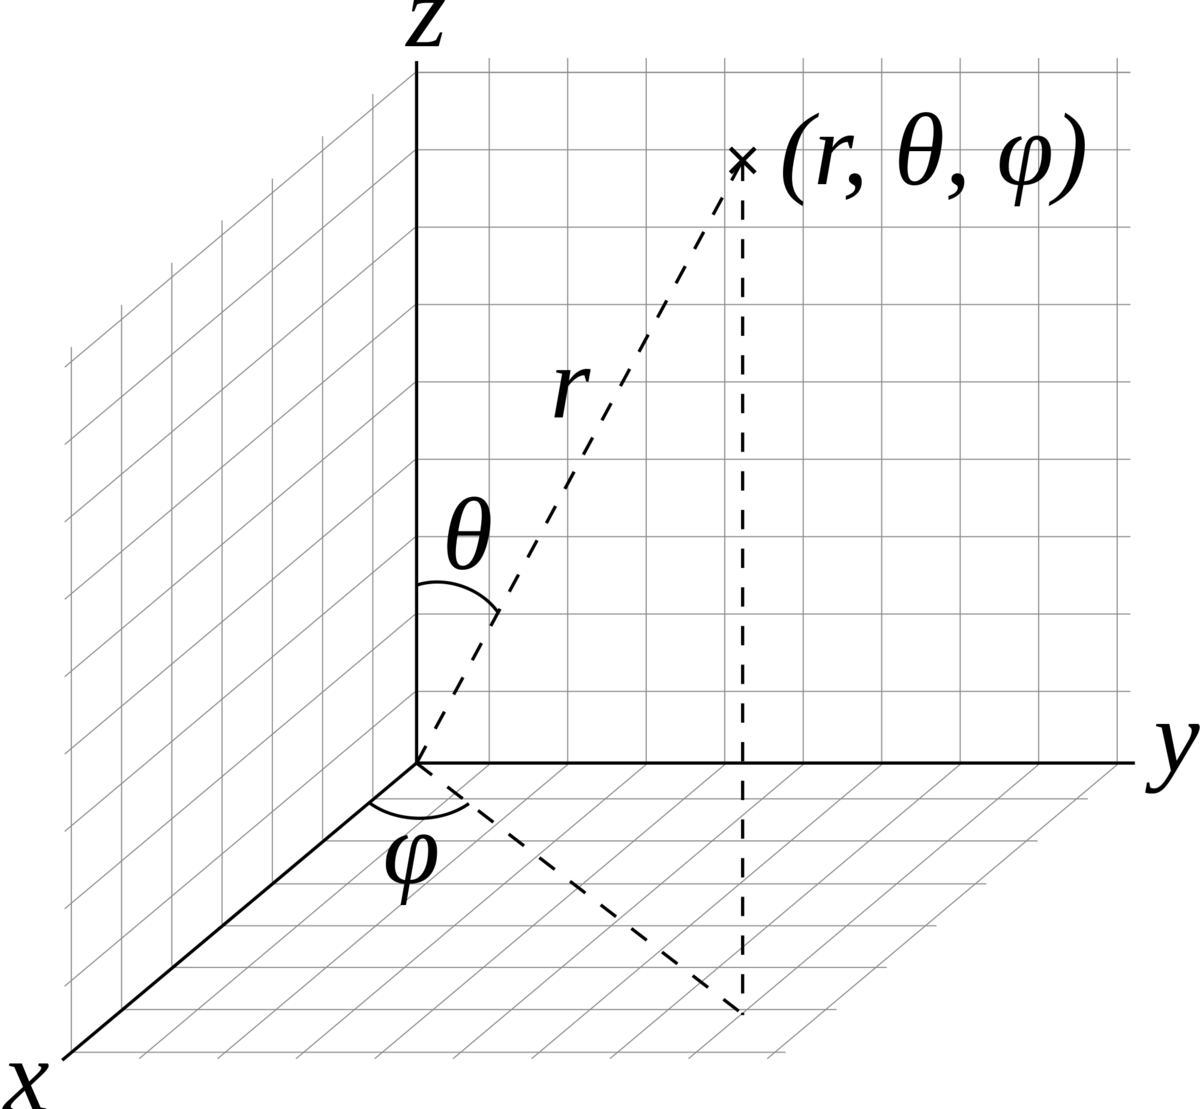
\includegraphics[width=5cm]{images/sphcoord}\\
{\captionfont Spherical coordinates as commonly used in physics:\\ polar angle $\theta$, and azimuthal angle $\phi$.} 
\end{center}
In this case $\theta\in[0:\pi]$ and $\phi\in]-\pi:\pi]$ and we have the following relationships:
\begin{eqnarray}
r &=& \sqrt{x^2+y^2+z^2} \\
\theta &=& \arccos (z/r) \\
\phi &=& \arctan (y/x) \\
x &=& r \sin \theta \cos \phi \\
y &=& r \sin\theta \sin\phi \\
z &=& r \cos\theta 
\end{eqnarray}
The inverse tangent used to compute $\phi$ must be suitably defined, 
taking into account the correct quadrant of $(x,y)$,
which is why the atan2 intrinsic function is used in fortran for example.    
This is often written as follows:
\begin{eqnarray}
\theta &=& \arctan \left(\sqrt{x^2+y^2},z\right) \\
\phi &=& \arctan (y,x) 
\end{eqnarray}
where we formally take advantage of the two argument arctan
function to eliminate quadrant confusion.

The path increment is expressed as:
\[
d\vec{r} = dr \; \vec{e}_r + r d\theta \; \vec{e}_\theta + r \sin\theta d\phi \; \vec{e}_\phi
\]
The gradient is 
\[
\vec\nabla = \frac{\partial}{\partial r} \; \vec{e}_r
+ \frac{1}{r} \frac{\partial}{\partial \theta} \; \vec{e}_\theta 
+ \frac{1}{r \; \sin\theta} \frac{\partial}{\partial \phi} \;  \vec{e}_\phi
\]
The divergence of a vector $\vec{V}$ is given in Eq.~\eqref{eq:divsc}. \index{general}{Divergence}
The Laplacian is given by: \index{general}{Laplacian}
\[
\Delta = \vec\nabla \cdot\vec\nabla = \vec\nabla^2
=
\frac{1}{r^2}\frac{\partial}{\partial r} \left( r^2 \frac{\partial}{\partial r} \right)
+\frac{1}{r^2 \sin\theta} \frac{\partial}{\partial \theta} \left( \sin\theta \frac{\partial}{\partial \theta} \right)
+\frac{1}{r^2 \sin^2\theta}  \frac{\partial^2}{\partial \phi^2}
\]




In geography one uses latitude and longitude, represented hereunder:
\begin{center}
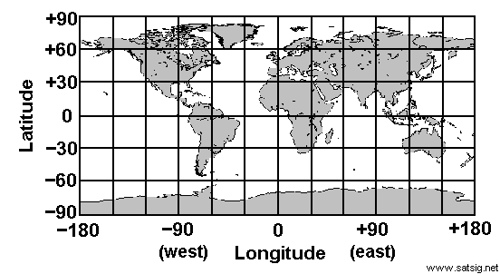
\includegraphics[width=10cm]{images/map.jpg}
\end{center}
\begin{itemize}
\item Latitude  $\in[-90:90]$,   or $\in[-\pi/2:\pi/2]$ 
\item Longitude $\in]-180:180]$, or $\in]-\pi:\pi]$ 
\end{itemize}

Since the colatitude is the complementary angle of the latitude, 
i.e. the difference between 90 and the latitude, 
where southern latitudes are denoted with a minus sign,
$\theta$ as shown above is actually is the colatitude.
The co-latitude is shown in red on the following figure:
\begin{center}
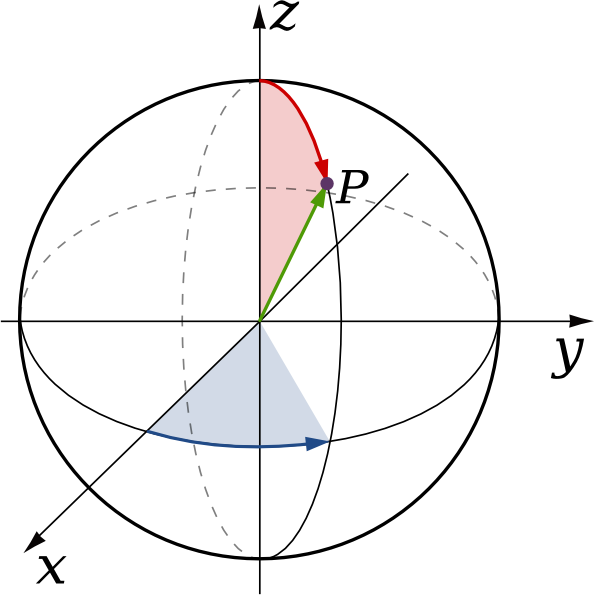
\includegraphics[width=3cm]{images/colatitude}
\end{center}

The volume of a sphere of radius $R$ is easily obtained by computing 
\begin{eqnarray}
V 
&=& \int dV \nn\\
&=& \int_0^R r^2 dr \int_0^\pi \sin\theta d\theta \int_0^{2\pi} d\phi  \nn\\
&=& \frac{1}{3}R^3  \cdot 2 \cdot 2\pi \nn\\
&=& \frac{4}{3}\pi R^3 
\end{eqnarray}

The spherical unit vectors are related to the cartesian unit vectors by:
\[
\left(
\begin{array}{c}
\vec{e}_{r} \\ \vec{e}_\theta \\ \vec{e}_\phi
\end{array}
\right)
=
\left(
\begin{array}{ccc}
\sin\theta \cos\phi & \sin\theta\sin\phi & \cos\theta  \\
\cos\theta \cos\phi & \cos\theta\sin\phi & -\sin\theta \\
-\sin\phi & \cos\phi & 0
\end{array}
\right)
\left(
\begin{array}{c}
\vec{e}_{x} \\ \vec{e}_y \\ \vec{e}_z
\end{array}
\right)
\]
and the cartesian unit vectors are related to the spherical unit vectors by

\[
\left(
\begin{array}{c}
\vec{e}_{x} \\ \vec{e}_y \\ \vec{e}_z
\end{array}
\right)
=
\left(
\begin{array}{ccc}
\sin\theta \cos\phi & \cos\theta\cos\phi & -\sin\phi  \\
\sin\theta \sin\phi & \cos\theta\sin\phi & \cos\phi \\
\cos\theta & -\sin\theta & 0
\end{array}
\right)
\left(
\begin{array}{c}
\vec{e}_{r} \\ \vec{e}_\theta \\ \vec{e}_\phi
\end{array}
\right)
\]

\begin{eqnarray}
\vec{\upnu} 
&=& u \vec{e}_x + v \vec{e}_y + w \vec{e}_z \\
&=& u ( \sin\theta \cos\phi \vec{e}_r +  \cos\theta\cos\phi \vec{e}_{\theta} -\sin\phi \vec{e}_{\phi} ) \\
&+& v ( \sin\theta \sin\phi \vec{e}_r + \cos\theta\sin\phi \vec{e}_\theta  +  \cos\phi \vec{e}_\phi  )  \\
&+& w ( \cos\theta \vec{e}_r   -\sin\theta \vec{e}_\theta  ) \\
&=& v_r \vec{e}_r + v_\theta \vec{e}_\theta + v_\phi \vec{e}_\phi 
\end{eqnarray}
with 
\begin{eqnarray}
v_r      &=&  u \sin \theta  \cos \phi  + v \sin\theta \sin \phi + w \cos\theta \\
v_\theta &=&  u \cos\theta\cos\phi + v \cos\theta\sin\phi -w \sin\theta   \\
v_\phi   &=& -u \sin\phi  + v \cos\phi  
\end{eqnarray}


